\documentclass[10pt]{beamer}
\usetheme{AAUsimple}

\usepackage[utf8]{inputenc}
\usepackage[T1]{fontenc}
\usepackage[danish]{babel}
\usepackage{helvet}
\usepackage{listings}

\newcommand{\chref}[2]{%
  \href{#1}{{\usebeamercolor[bg]{AAUsimple}#2}}%
}


\author{}
\institute{
  Institut for Matematiske Fag\\
  Aalborg Universitet\\
  Danmark

}
\pgfdeclareimage[height=1.5cm]{titlepagelogo}{AAUgraphics/aau_logo_new}
\titlegraphic{\pgfuseimage{titlepagelogo}}


\title{Projektsamarbejde med Git}
\subtitle{Workshop 4}
\date{16. september 2019}

\begin{document}

% Title page
{\aauwavesbg
  \begin{frame}[plain,noframenumbering]
    \titlepage
  \end{frame}}

% TOC
\begin{frame}{Agenda}
  \tableofcontents
\end{frame}

\section{Om versionsstyring}
\label{sec:about}

\begin{frame}{Versionsstyring, kort fortalt}
  \begin{block}{Hvorfor bruge versionsstyring?}
    \begin{itemize}
    \item Gør gruppearbejde nemmere
    \item Ordnet historik over filændringer
    \item Mulighed for at rulle individuelle ændringer tilbage
    \item Fuld backup af alle versioner af projektet
    \item ``Do What I Say''---ingen pludselige automatiske synkroniseringer, intet mistet arbejde
    \item Indbygget konflikthåndtering
    \end{itemize}
  \end{block}
\end{frame}

\begin{frame}{Versionsstyring, kort fortalt}
  \begin{block}{Git}
    \begin{itemize}
    \item Mest brugte (men ikke eneste) versionsstyringssystem

      \(\implies\) man kan finde løsninger til alle problemer online
    \item Letvægt og hurtigt
    \item Fleksibel, mange forskellige workflows
    \item GitHub
    \end{itemize}
  \end{block}

  \begin{block}{\url{https://git-scm.com}}
  \end{block}
\end{frame}

\begin{frame}{GitAhead}{Grafisk brugerflade til Git}
  \begin{center}
    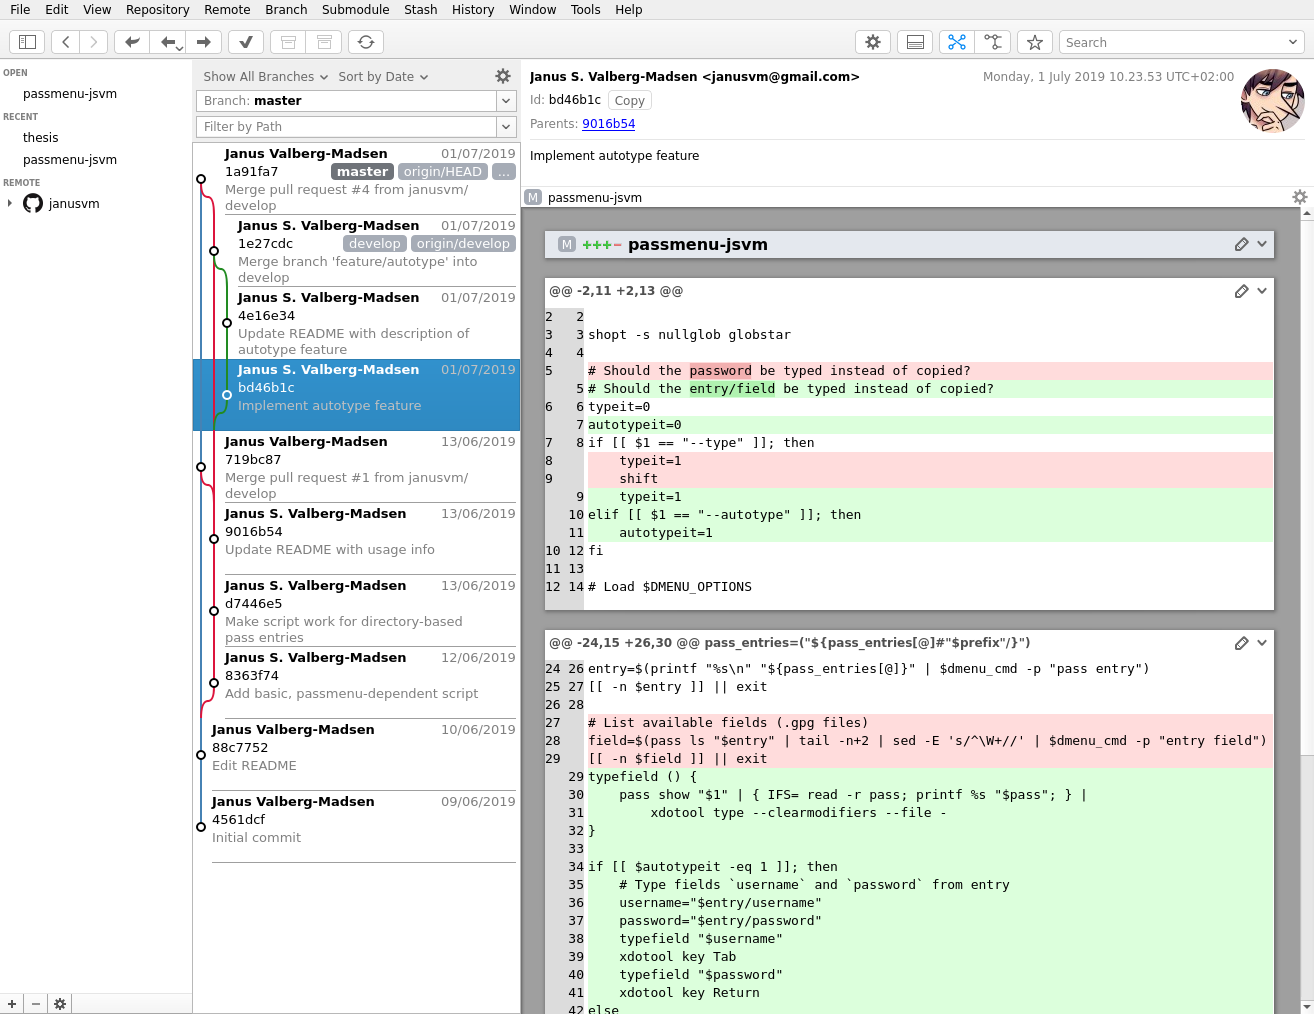
\includegraphics[width=0.8\textwidth]{img/gitahead}
  \end{center}
\end{frame}

\begin{frame}{GitAhead}{Grafisk brugerflade til Git}
  \begin{block}{\url{https://gitahead.com}}
    \begin{itemize}
    \item Fri og open source software
    \item Multiplatform (GNU/Linux, macOS, Windows)
    \item Integration med GitHub
    \item Vigtigste værktøjer let tilgængelige
    \item Alternativer: \url{https://git-scm.com/downloads/guis}
    \end{itemize}
  \end{block}
\end{frame}

\section{Overblik over Git}
\label{sec:gitcmds}

\begin{frame}{Funktioner i Git}
  \begin{minipage}[t]{0.3\textwidth}
    \begin{block}{Info}
      \begin{itemize}
      \item \texttt{status}
      \item \texttt{log}
      \end{itemize}
    \end{block}
  \end{minipage}
  \begin{minipage}[t]{0.3\textwidth}
    \begin{block}{Lokal}
      \begin{itemize}
        \ttfamily
      \item add
      \item reset
      \item commit
      \item revert
      \item checkout
      \end{itemize}
    \end{block}
  \end{minipage}
  \begin{minipage}[t]{0.3\textwidth}
    \begin{block}{Server}
      \begin{itemize}
      \item \texttt{clone}
      \item \texttt{pull}
      \item \texttt{push}
      \end{itemize}
    \end{block}
  \end{minipage}

  \begin{block}{}
    Lad os se på nogle eksempler i GitAhead
  \end{block}
\end{frame}

\section{\LaTeX-skabelon}
\label{sec:template}

\begin{frame}{\LaTeX-skabelon}{Kom hurtigt i gang med \LaTeX\ og GitHub}
    \begin{enumerate}
    \item Log ind på github.com
    \item Følg en af nedenstående links for at bruge den pågældende skabelon:

      {\footnotesize\url{https://github.com/janusvm/aau-project-template-danish/generate}}
      {\footnotesize\url{https://github.com/janusvm/aau-project-template-english/generate}}

    \item Giv projektet en titel, f.eks.\ \texttt{P1}
    \item Hvis du har fået din student discount, sæt projektet til \textbf{Private}
    \item Tryk på \textbf{Generate repository from template}
    \item Tryk på \textbf{Settings}-fanen øverst til højre
    \item Tryk på \textbf{Collaborators}-sektionen til venstre
    \item Skriv en efter en dine gruppemedlemmers brugernavne ind og tryk \textbf{Add collaborator}
    \item Klon til din computer, og du er i gang!
    \end{enumerate}
\end{frame}

\end{document}
